\chapter{Vergleich}
\label{cha:Vergleich}

Folgend wird zur Darstellung des Entwicklungsprozesses, und der Unterschiede zwischen der konventionellen prozeduralen Entwicklung in C/AL, und der erweiterungsbasierten Entwicklung in AL ein Beispiel in beiden Sprachen entwickelt.


\section{Aufgabenstellung}
\label{sec:Aufgabenstellung}

Für die Kunden des Auftraggebers unserer Erweiterung sollen Treuepunkte verwaltet werden. Treuepunkte werden mit dem Kauf von Waren verdient, oder von der Marketingabteilung an Bestandskunden vergeben. Treuepunkte können beim Kauf von Produkten eingelöst werden, um einen Preisnachlass zu erzielen. Eingelöste Punkte verringern den Rechnungsbetrag um einen bestimmten Geldwert, der variieren kann. So mag ein Treuepunkt im Januar 10 Cent wert sein, im Februar jedoch 15 Cent. Die Schwankung des Treuepunktwertes wird als Marketinginstrument genutzt. Auch wie viele Treuepunkte beim Einkauf vergeben werden ist variabel, so sind etwa Aktionszeiträume vorgesehen, in denen beim Einkauf doppelt so viele Treuepunkte verdient werden können.
\linebreak

Das neue Treuepunktesystem ist für das Marketing von hoher Bedeutung. So ist es erforderlich, dass Änderungen am Treuepunktekonto eines Kunden über einen Web Service an das verwendete CRM-System gemeldet werden. Für das Reporting im Unternehmen ist es außerdem nötig, dass täglich ein XML Datenträger erzeugt werden kann, in dem der Treuepunktesaldo und die Bewegungen des aktuellen Tages je Kunde ersichtlich sind. Zusätzlich zu dieser Datei für das Berichtssystem soll auch ein übersichtlicher Ausdruck in PDF-Form an die Marketingleitung gesendet werden.
\pagebreak

\section{Entwicklungsprozess}
\label{sec:Entwicklungsprozess}

\subsection{Entwicklungsumgebung}
\subsubsection{C/AL - Development Environment}
C/AL wird im \textit{Microsoft Dynamics Development Environment} entwickelt. Dabei handelt es sich eigentlich um den Client, der bis zur Version 2009 noch als Windows Client für Endbenutzer verwendet wurde, nun seit dem jedoch rein für die Entwicklung genutzt wird. Das Development Environment ist ein Windows Client, der stets sowohl mit Datenbank, als auch mit der Serverapplikation verbunden sein muss. Die Datenbankverbindung ist nötig, da darin die Applikationsobjekte gespeichert sind, die Verbindung zum Applikationsserver, um Änderungen kompilieren und Ausführen zu können.
\linebreak

Das Kernstück des Development Environment bildet der \textit{Object Designer}. Der \textit{Object Designer} liefert einen Überblick über sämtliche, im System vorhanden Applikationsobjekte und Details zu Ihnen. Ein Applikationsobjekt unter C/AL wird durch eine numerische ID und seinen Namen identifiziert. Zusätzlich wird zu den einzelnen Applikationsobjekten auch

\begin{figure}[h]
	\centering
	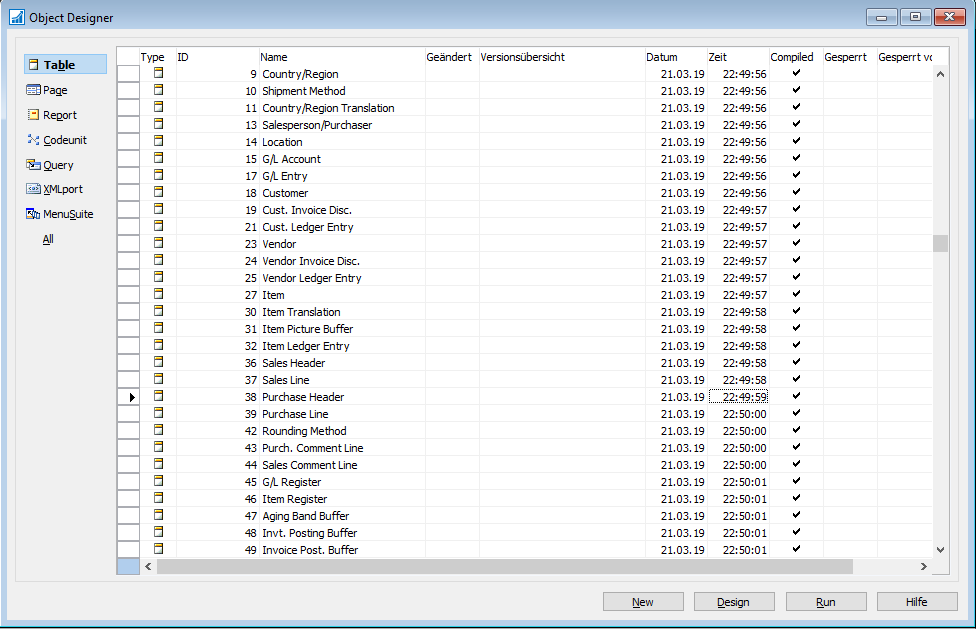
\includegraphics[width=130mm]{images/ObjectDesigner}
	\caption{Development Environment: Object Designer und C/AL Editor}
	\label{fig:ObjectDesigner}
\end{figure}

Je nach ausgewählter Objektart stellt das Development Environment einen auf die Objektart angepassten \textit{Designer} zur Verfügung, über den bereits einige Basiseinstellungen getätigt werden können. Über den Designer gelangt man ebenfalls zum C/AL Editor, in dem dann die wirkliche Programmierung stattfindet.

\begin{figure}[h]
	\centering
	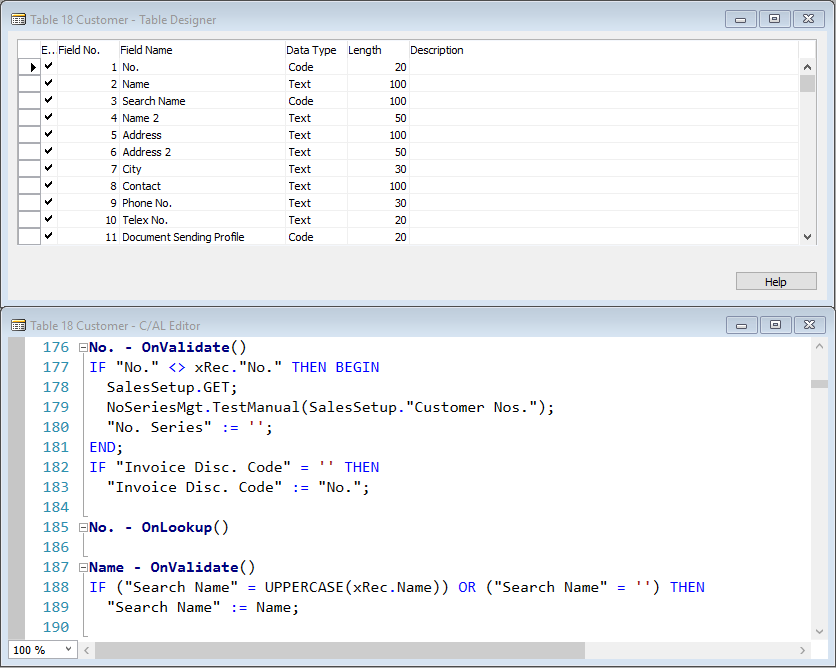
\includegraphics[width=130mm]{images/TableDesigner}
	\caption{Development Environment: Table Designer und C/AL Code Editor}
	\label{fig:TableDesignerCodeEditor}
\end{figure}

\subsubsection{AL - Visual Studio Code}